 
% ME3001   
% Tristan Hill - Spring 2024 
% Systems of Linear Equations 
% Simple Truss Analysis


% Document setting
\documentclass[11pt]{article}
\usepackage[margin=1in]{geometry}
\usepackage[pdftex]{graphicx}
\usepackage{multirow}
\usepackage{setspace}
\usepackage{hyperref}
\usepackage{color,soul}
\usepackage{fancyvrb}
\usepackage{framed}
\usepackage{wasysym}
\usepackage{multicol}

\pagestyle{plain}
\setlength\parindent{0pt}


% assignment number 
\newcommand{\NUM}{3} 
\newcommand{\HSPC}{42mm} 
\newcommand{\HHSPC}{33mm} 
\newcommand{\VSpaceSize}{2mm} 
\newcommand{\HSpaceSize}{2mm} 

\definecolor{mygray}{rgb}{.6, .6, .6}

% [153,50,204] - dark orchid
\definecolor{mypurple}{rgb}{0.6,0.1961,0.8}
%[139,69,19] - saddle brown
\definecolor{mybrown}{rgb}{0.5451,0.2706,0.0745}


\begin{document}

	\textbf{\LARGE ME3001 - Spring 2024} \\\\
	\textbf{\LARGE Weekly Activity \NUM:  Systems of Linear Equations}\\\\
	\textbf{\LARGE Static Analysis of a Simple Truss} \\
	
	\begin{description}


\item[\textbf{\underline{Learning Objectives:}}] \hfill \vspace{0mm}

\begin{itemize}
  \item Demonstrate deriving a system of ,linear equations to represent a static analysis.
  \item Demonstrate converting a system of linear equations into matrix form.
  \item Practice using linear algebra techniques in MATLAB to solve an applied engineering problem.
\end{itemize}


\item[\textbf{\underline{Overview:}}] \hfill \vspace{3mm}\\

As an engineer you are asked to analyze the simple scaffolding structure shown. The rigid structure above rests on the ground in static equilibrium. 

\item[\textbf{\underline{Overview:}}] \hfill \vspace{3mm}\\
  
    
  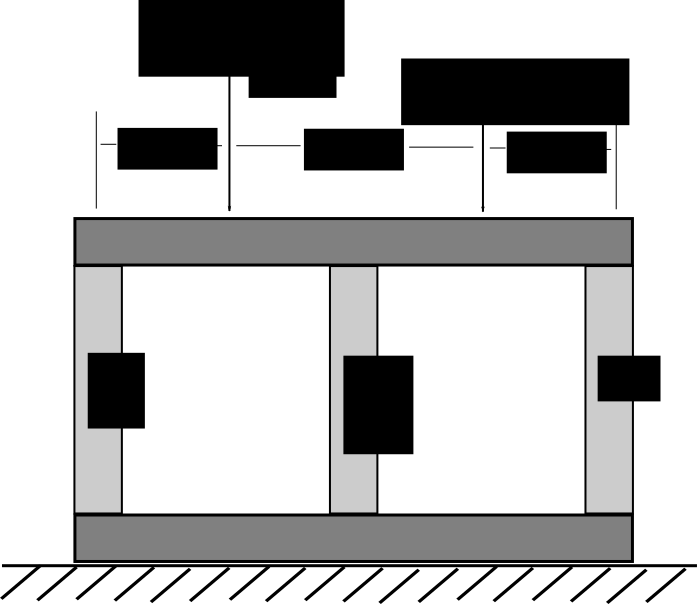
\includegraphics[scale=.25]{quiz2_fig1.png}\\
    
  \item[\textbf{\underline{Peer Collaboration:}}] \hfill \vspace{0mm}
  
  {\bf This is an individual assignment}, but you are encouraged to discuss the problem with your peers. You must write your own program and submit as an individual, but you can share ideas about the algorithm with your peers and the instructor.

\newpage  
\item[\textbf{\underline{Analysis Requirements:}}] \hfill \vspace{0mm}

  
  \begin{itemize}
    
  \item Write 2 static equilibrium equations for ASDF and ASDF each for a total of 4 equations. Show the equations with unknowns in order and the knowns on the right hand side.\vspace{10mm} \\
  
  %   \scalebox{1}{$KVL_1=-v_a+R_1\times i_1-(i_1-i_2)\times R_2 =0$} \vspace{3mm} \vspace{30mm}
  
  \item Cast the system of equations into matrix form. Be sure to label the {\it Coefficient Matrix}, {\it The Vector of Knowns}, and {\it The Vector of Unknowns}. Also, please write the unknown vector with the loads in order (1,2,3,4).\vspace{10mm}
  
  
  \item Solve for the unknowns using the matrix inverse. 
  
  \end{itemize}


\item[\textbf{\underline{Activity:}}] \hfill \vspace{0mm}

\begin{enumerate}
  

  \item Write a MATLAB program to solve the static analysis problem described on the previous page. Include a decriptive title block at the top of your main program. 
  
  
  \item Write a brief description of how your program works to solve the problem. This can be a few sentences or a bulleted list.
  
  
\end{enumerate}


  \item [\textbf{ \large Deliverables}] \textbf{ \Large :}\\
    \begin{itemize} 
   
      \item MATLAB Code:
Write a MATLAB program use a method of your choice to solve the given problem. The solution strategy should be clearly defined and documented. Submit the .m file(s) used and document any example code that you used or learned from during the exercise.

      \item Results:
Submit a brief summary of the problem statement and present the results from the solution code. The results can be typed in the program comments or typed in the assignment text box.

    \end{itemize}
  \end{description}
 
\end{document}



